\ifpdf
    \graphicspath{{figures/}{figures/comparisons}}
\else
    \graphicspath{{figures/}{figures/comparisons}}
\fi
% this file is called up by thesis.tex
% content in this file will be fed into the main document

\chapter{Additional materials} % top level followed by section, subsection
\begin{lstlisting}[language=json,firstnumber=1, float, label={lst:json_file} caption=Sample ''sensor.txt'' file from ''Sensor Enhanced Images Camera'' application]
[
   {
      "photoPath":"20141210_145643/0.jpg",
      "rotationMatrix":[],
      "azimuth":121.88075,
      "posX":-1.7521392107009888,
      "posY":-1.4345977306365967,
      "posZ":0.9248641133308411,
      "photoId":1,
      "pitch":13.867888,
      "roll":178.16968
   },
   {
      "photoPath":"20141210_145643/1.jpg",
      "rotationMatrix":[],
      ],
      "azimuth":110.66925,
      "posX":-4.244707942008972,
      "posY":-1.1443554759025574,
      "posZ":0.9647054933011532,
      "photoId":2,
      "pitch":11.625216,
      "roll":179.73383
   }
   ...
]
\end{lstlisting} %TODO opis i caption z referencją do implementation
\clearpage

\begin{table}[p]
\centering
\begin{adjustbox}{width=1\linewidth}
\begin{tabular}{l|l|l|l|l}
\textbf{100 SIFT Features}   & \textbf{Total Sampson Error} & \textbf{Sampson Error per Point} & \textbf{Points left} & \textbf{Execution time(ms)} \\ \hline
\textbf{8-point OpenCV}      & 20.5793             & 0.478588                & 43          & 0.4387             \\ \hline
\textbf{Alternative 3-point} & 112.749             & 4.17588                 & 27          & 0.1484             \\ \hline
\textbf{8-point enhanced}    & 67.2559             & 1.56409                 & 43          & 0.3867             \\ \hline
\textbf{Known rot and trans} & 3501.23             & 83.3625                 & 42          & 0.0001             \\ \hline
\textbf{Essential 5-point}   & 43.5866             & 1.06309                 & 41          & 0.684              \\ \hline
\textbf{5-point enhanced}    & 1863.66             & 45.4552                 & 41          & 13.4643            \\
\end{tabular}
\end{adjustbox}
\caption[Efficiency table of proposed methods for 100 SIFT features in Warsaw University of technology dataset]{Efficiency table of proposed methods for 100 SIFT features in Warsaw University of technology dataset. Columns: Total Sampson Error, Average Sampson error per point, Amount of points left after outliers removal, Execution time}
\label{table:Efficiency100Sift}
\end{table}

\begin{table}[p]
\centering
\begin{adjustbox}{width=1\linewidth}
\begin{tabular}{l|l|l|l|l}
\textbf{500 SIFT features}   & \textbf{Total Sampson Error} & \textbf{Sampson Error per Point} & \textbf{Points left} \& \textbf{Execution time(ms)} \\ \hline
\textbf{8-point OpenCV}      & 100.584             & 0.543697                & 185         & 1.0833             \\ \hline
\textbf{Alternative 3-point} & 220.722             & 2.53704                 & 87          & 0.2692             \\ \hline
\textbf{8-point enhanced}    & 112.7               & 0.609189                & 185         & 0.8362             \\ \hline
\textbf{Known rot and trans} & 14770.7             & 80.2756                 & 184         & 0.0001             \\ \hline
\textbf{Essential 5-point}   & 404.098             & 2.29601                 & 176         & 3.8827             \\ \hline
\textbf{5-point enhanced}    & 501.987             & 2.8522                  & 176         & 47.0683            \\
\end{tabular}
\end{adjustbox}
\caption[Efficiency table of proposed methods for 500 SIFT features in Warsaw University of technology dataset]{Efficiency table of proposed methods for 500 SIFT features in Warsaw University of technology dataset. Columns: Total Sampson Error, Average Sampson error per point, Amount of points left after outliers removal, Execution time}
\label{table:Efficiency500Sift}
\end{table}

\begin{table}[p]
\centering
\begin{adjustbox}{width=1\linewidth}
\begin{tabular}{l|l|l|l|l}
\textbf{1000 SIFT features}  & \textbf{Total Sampson Error} & \textbf{Sampson Error per Point} & \textbf{Points left} & \textbf{Execution time(ms)} \\ \hline
\textbf{8-point OpenCV}      & 265.637             & 0.781287                & 340         & 1.5055             \\ \hline
\textbf{Alternative 3-point} & 640.895             & 4.1083                  & 156         & 0.4725             \\ \hline
\textbf{8-point enhanced}    & 295.152             & 0.868093                & 340         & 1.8099             \\ \hline
\textbf{Known rot and trans} & 27394.4             & 77.1673                 & 355         & 0.0001             \\ \hline
\textbf{Essential 5-point}   & 518.293             & 1.85768                 & 279         & 5.4482             \\ \hline
\textbf{5-point enhanced}    & 349.393             & 1.2523                  & 279         & 204.2998           \\
\end{tabular}
\end{adjustbox}
\caption[Efficiency table of proposed methods for 1000 SIFT features in Warsaw University of technology dataset]{Efficiency table of proposed methods for 1000 SIFT features in Warsaw University of technology dataset. Columns: Total Sampson Error, Average Sampson error per point, Amount of points left after outliers removal, Execution time}
\label{table:Efficiency1000Sift}
\end{table}

\begin{table}[p]
\centering
\begin{adjustbox}{width=1\linewidth}
\begin{tabular}{l|l|l|l|l}
\textbf{5000 SIFT features}      & \textbf{Total Sampson Error} & \textbf{Sampson Error per Point} & \textbf{Points left} & \textbf{Execution time(ms)} \\ \hline
\textbf{8-point OpenCV}          & 517.189             & 0.439413                & 1177        & 2.187              \\ \hline
\textbf{Alternative 3-point}     & 1879.98             & 3.28094                 & 573         & 0.8286             \\ \hline
\textbf{8-point enhanced}        & 1087.78             & 0.924199                & 1177        & 5.4395             \\ \hline
\textbf{Known rot and trans}     & 93951.1             & 77.9677                 & 1205        & 0.0001             \\ \hline
\textbf{Essential 5-point}       & 1949.53             & 1.95736                 & 996         & 15.2223            \\ \hline
\textbf{5-point enhanced}        & 19966.6             & 20.0468                 & 996         & 355.464            \\ 
\end{tabular}
\end{adjustbox}
\caption[Efficiency table of proposed methods for 5000 SIFT features in Warsaw University of technology dataset.]{Efficiency table of proposed methods for 5000 SIFT features in Warsaw University of technology dataset. Columns: Total Sampson Error, Average Sampson error per point, Amount of points left after outliers removal, Execution time}
\label{table:Efficiency5000Sift}
\end{table}

\begin{figure}[p]
    \centering
    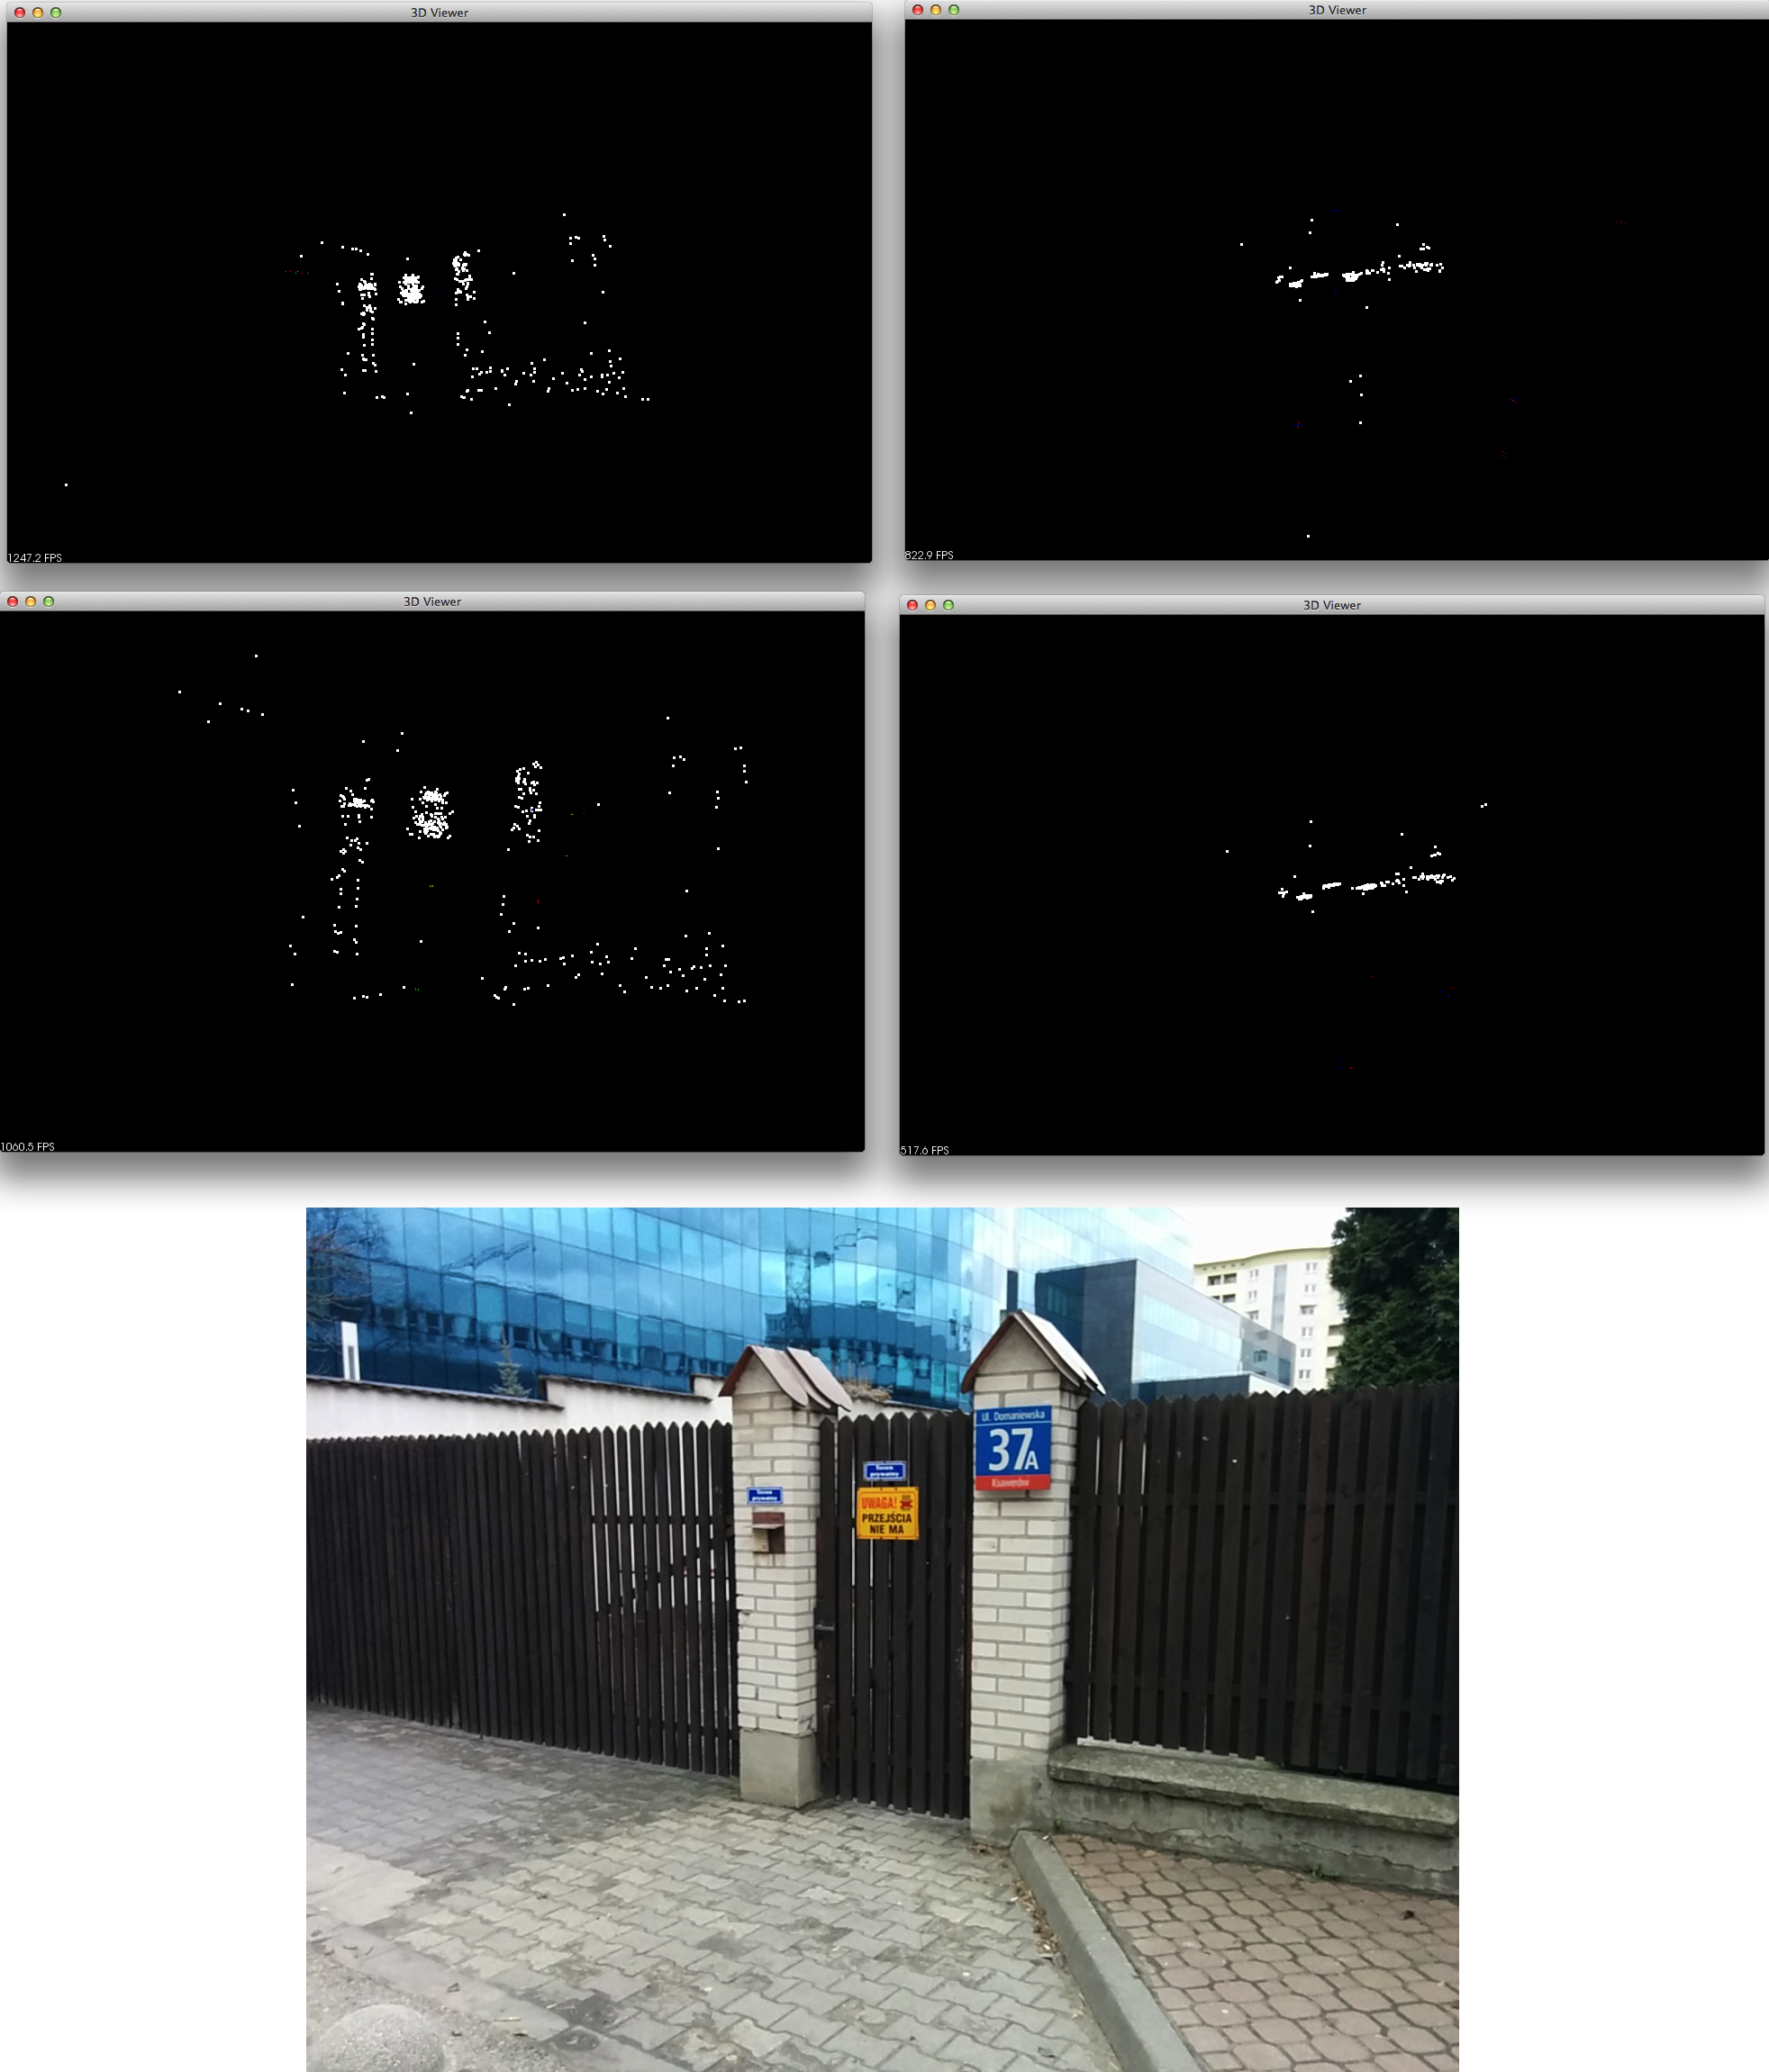
\includegraphics[height=18cm]{Gate4000Comparison}
    \caption[Reconstruction results of ''Gate'' dataset]{Reconstruction results of ''Gate'' dataset. Upper pair - standard OpenCV 8-point algorithm (left - front view, right - above view). Bottom pair - rotation enhanced 8-point algorithm.}
\end{figure}

\begin{figure}[p]
    \centering
    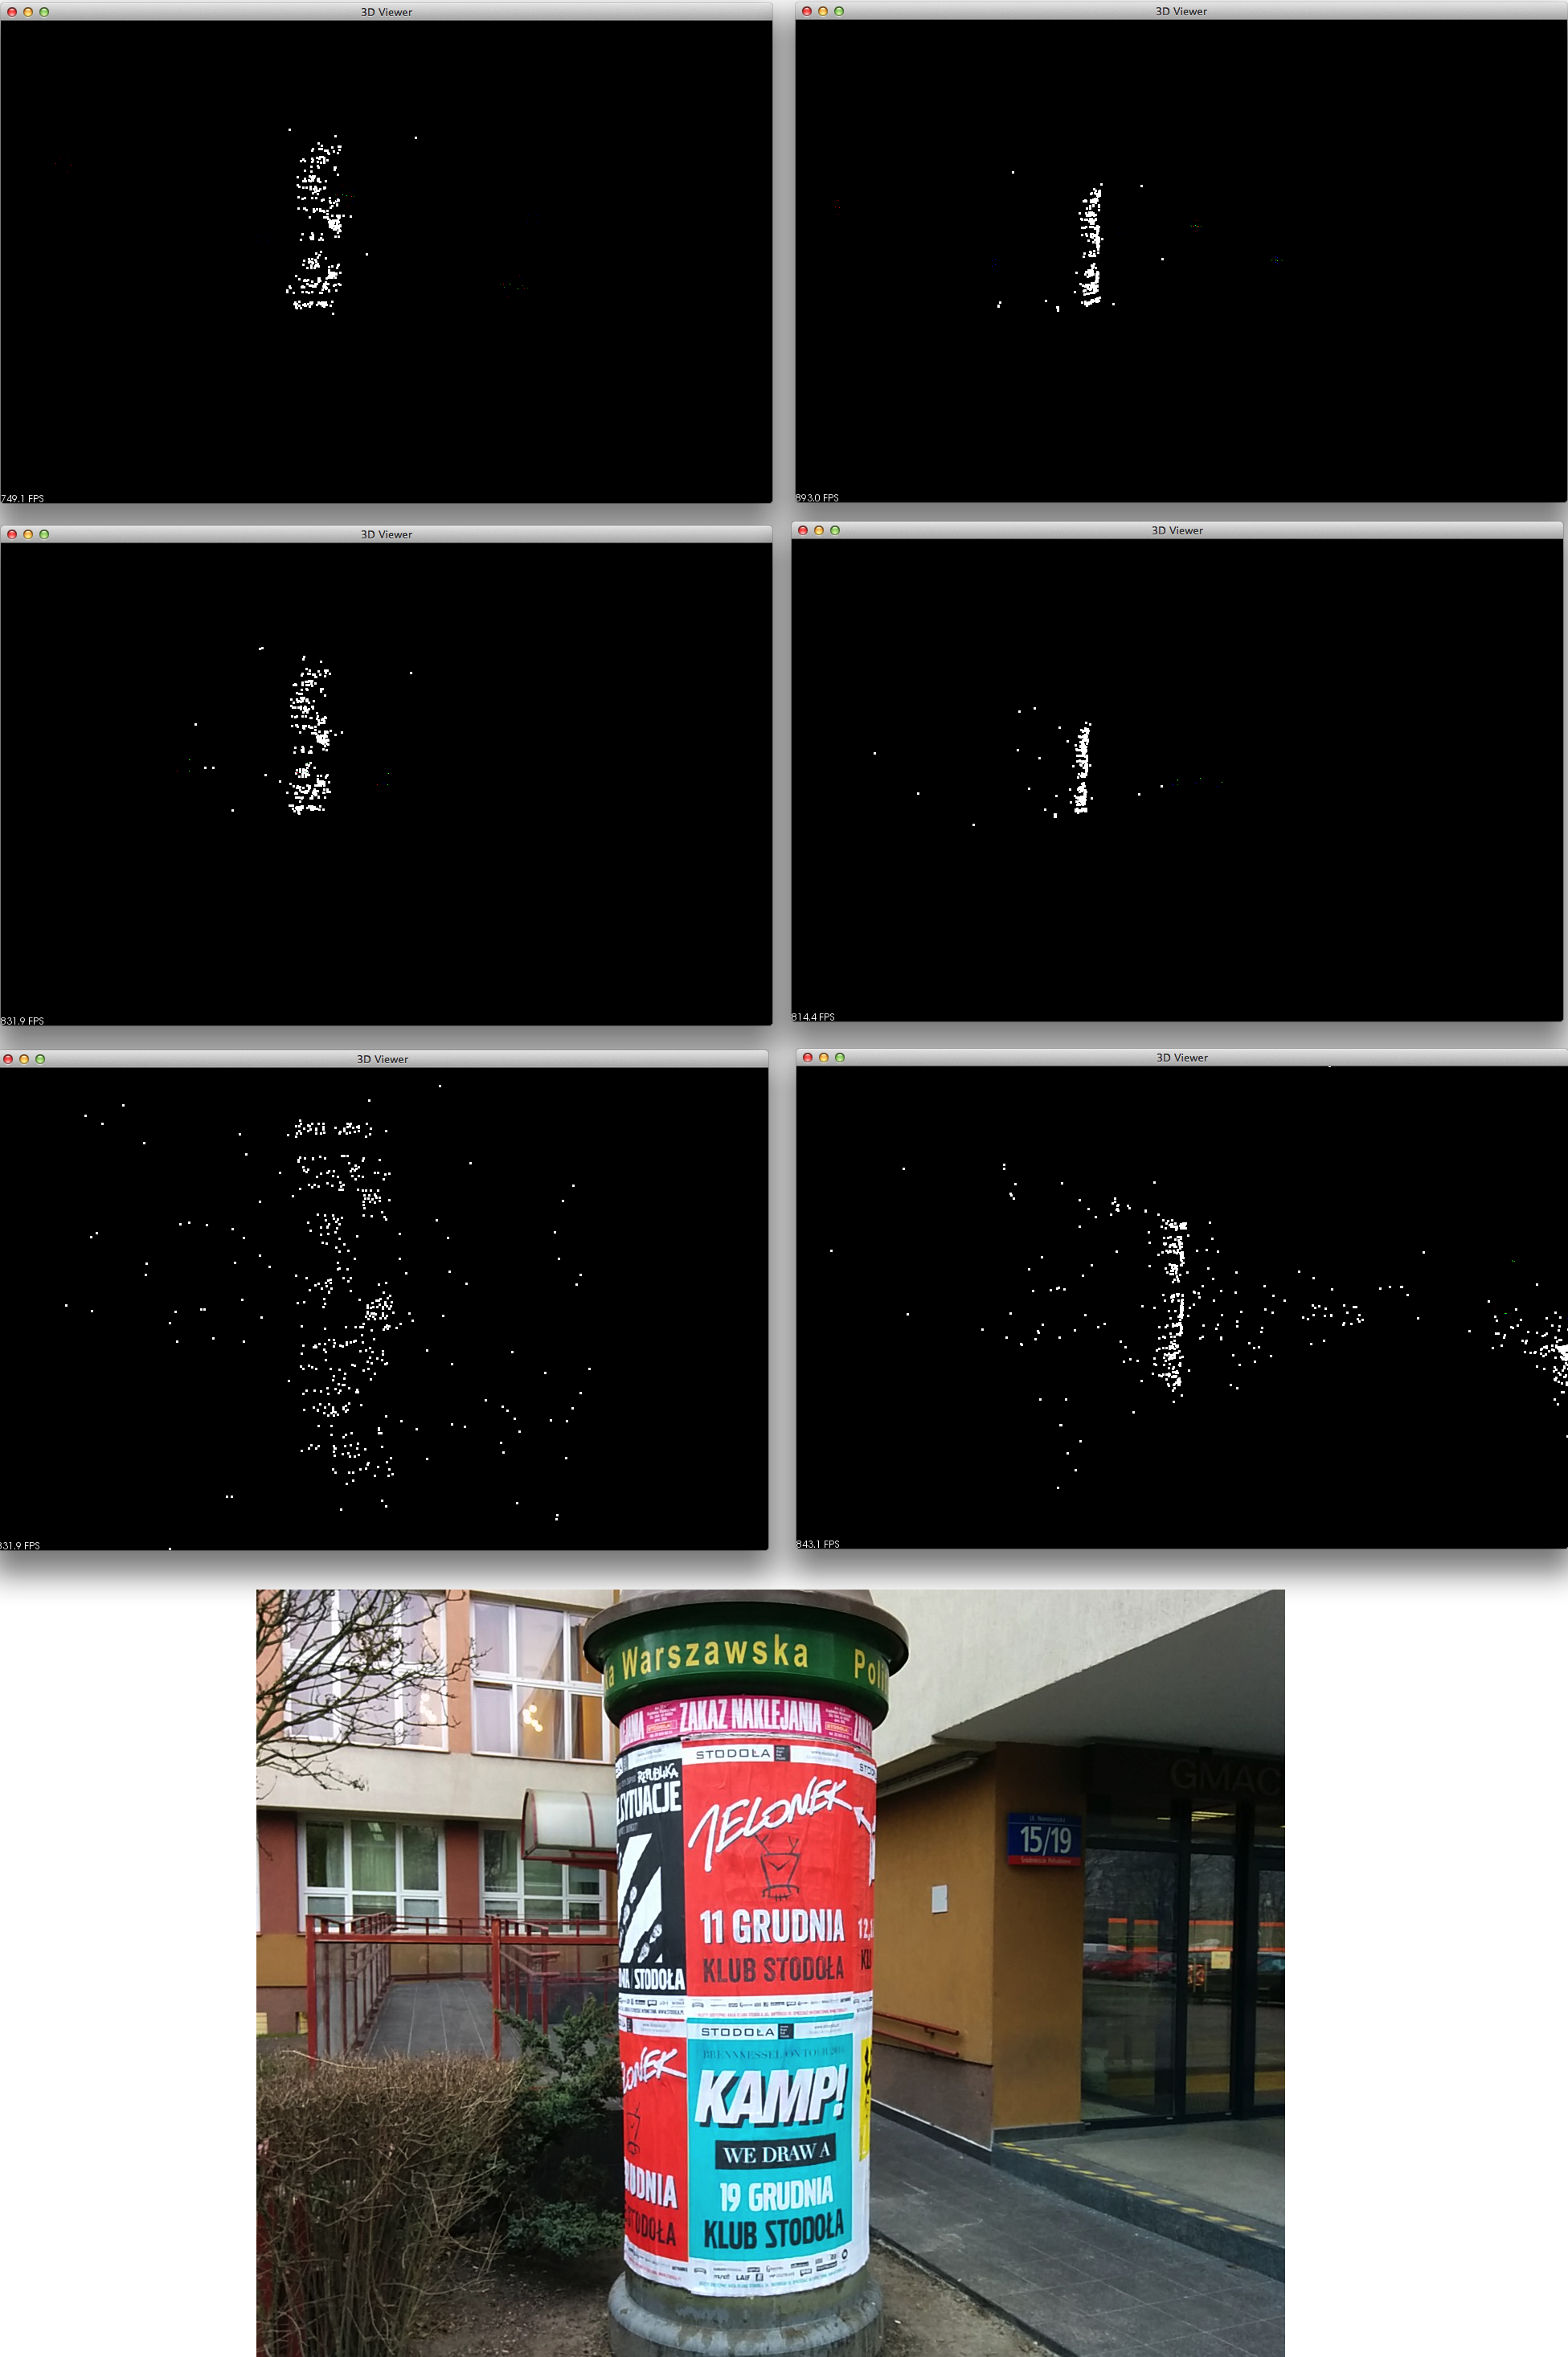
\includegraphics[height=18cm]{Pole4000Comparison}
    \caption[Reconstruction results of ''Pole'' dataset]{Reconstruction results of ''Pole'' dataset. Upper pair - standard OpenCV 8-point algorithm (left - front view, right - above view). Middle pair - rotation enhanced 8-point algorithm. Bottom pair - reconstruction from known rotations and translations.}
\end{figure}

\begin{figure}[p]
    \centering
    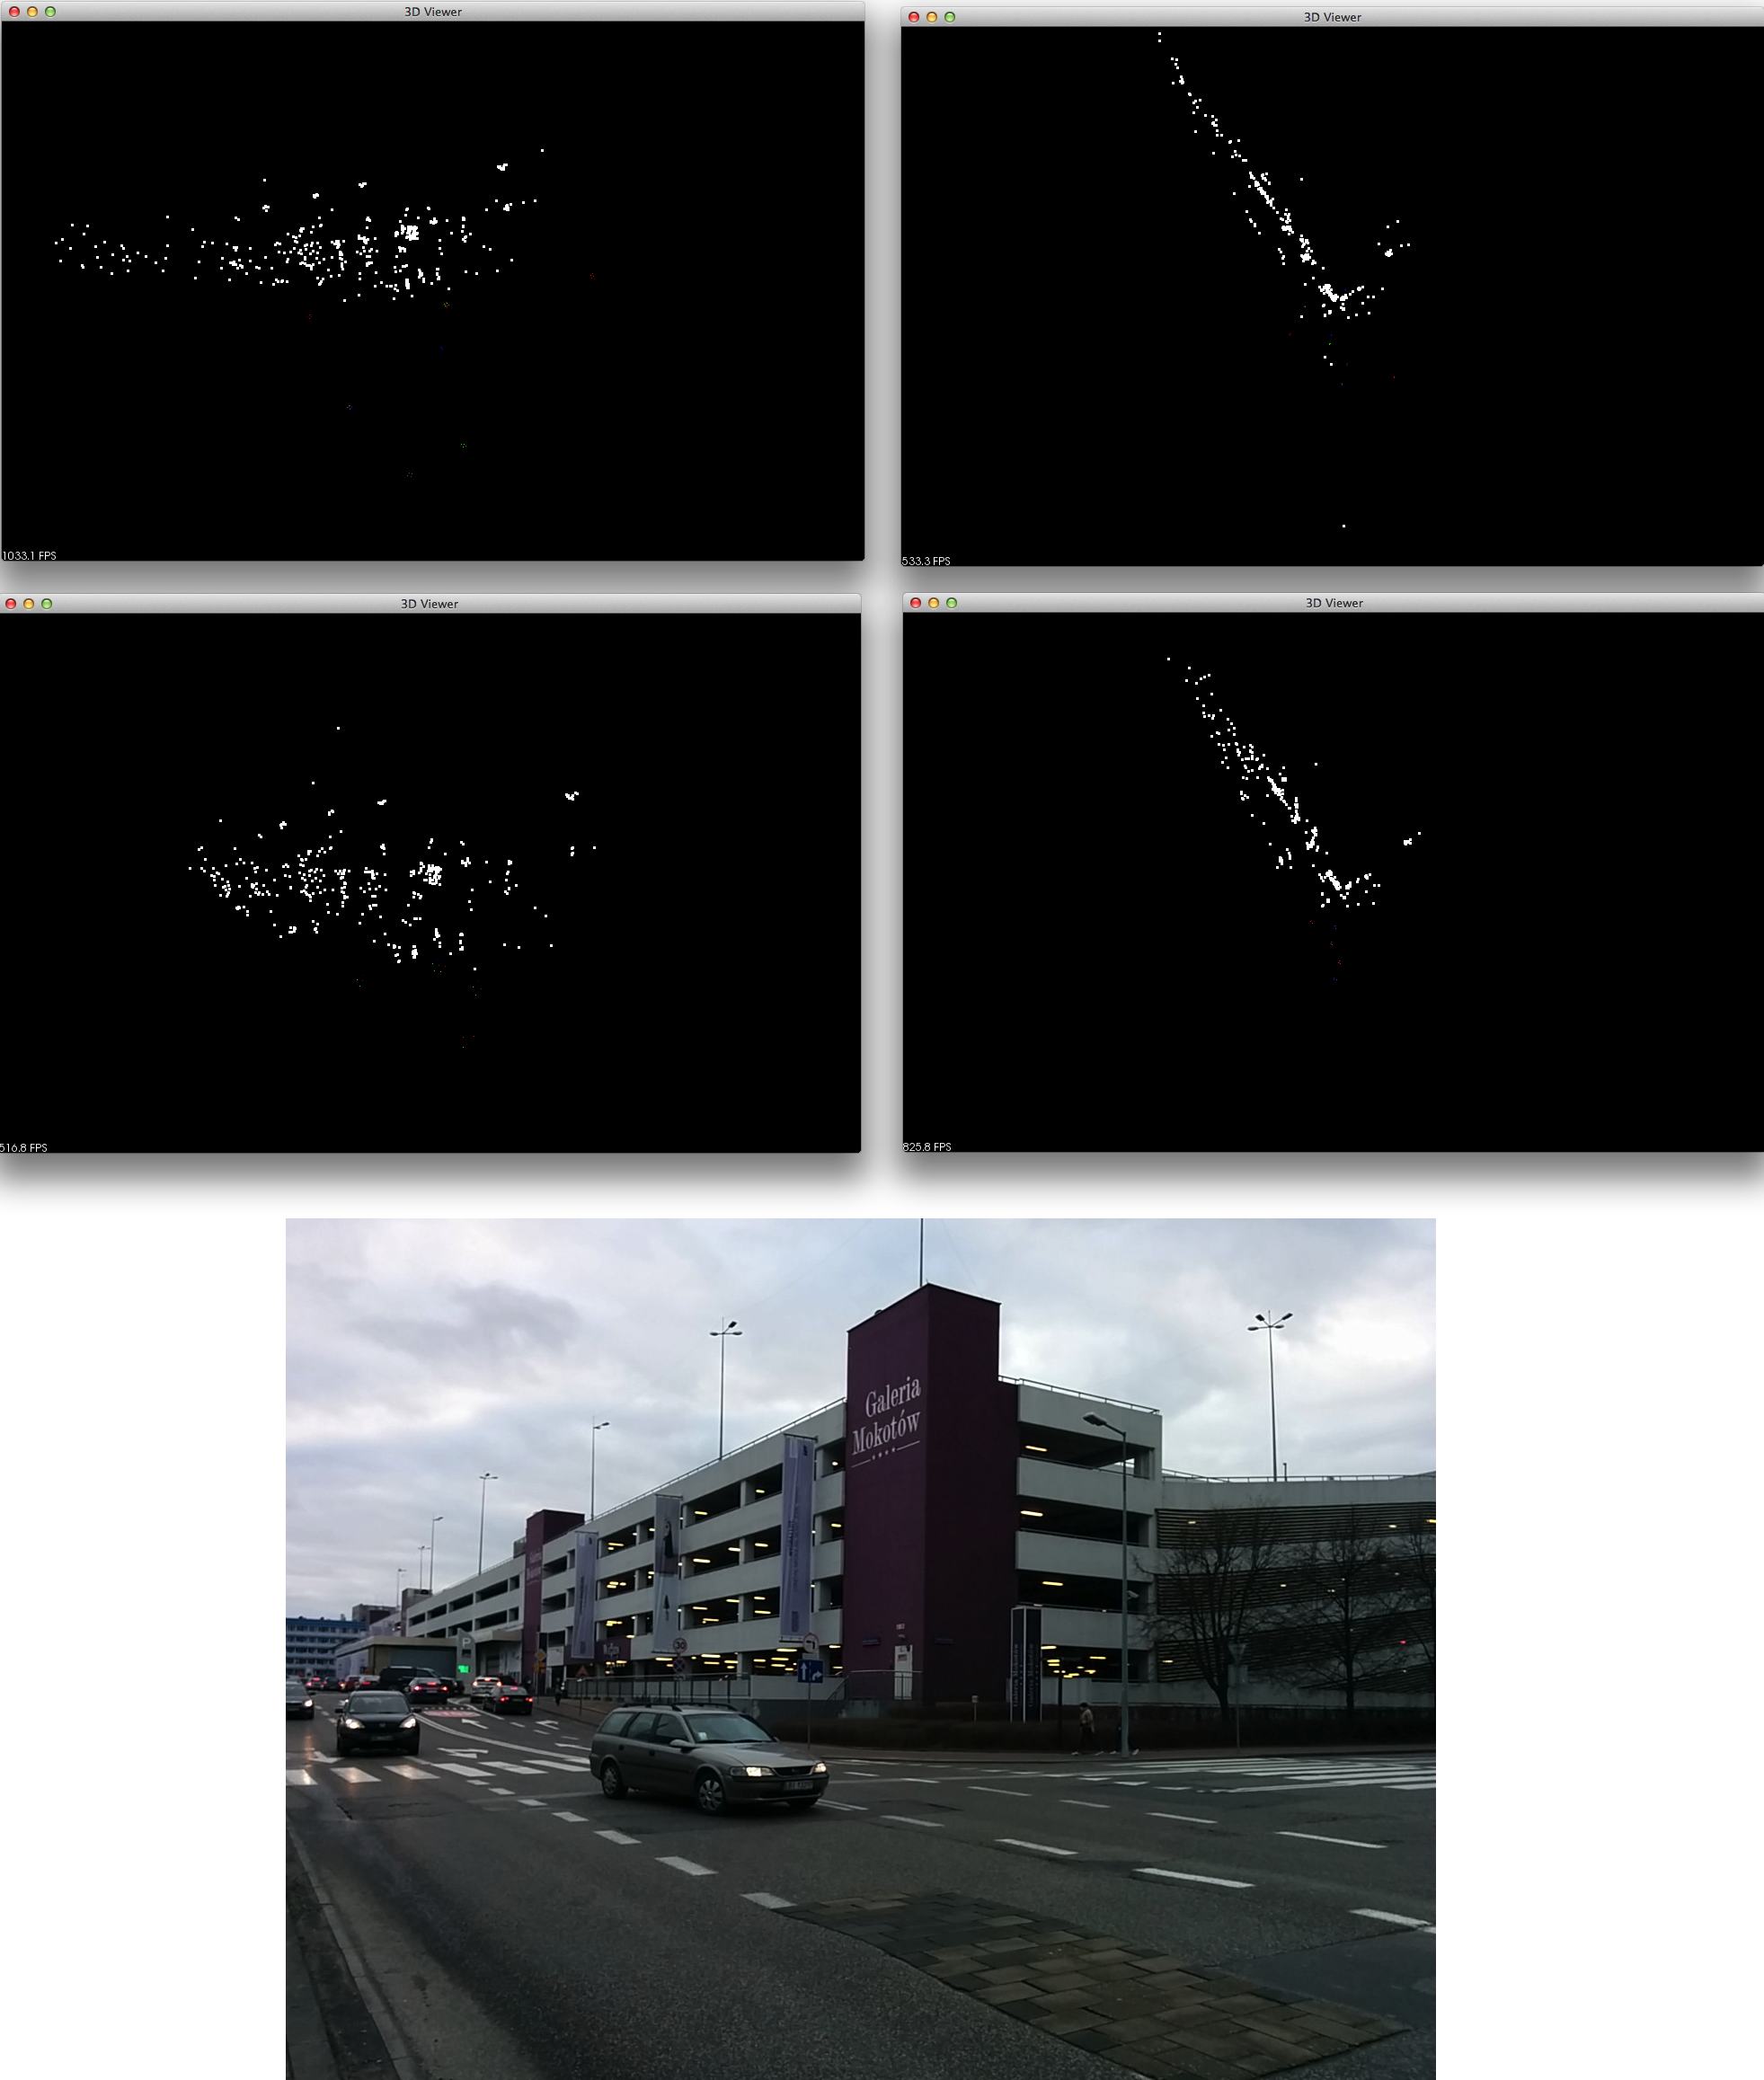
\includegraphics[height=18cm]{GalleryBack4000Comparison}
    \caption[Reconstruction results of ''Gallery Back'' dataset]{Reconstruction results of ''Gallery Back'' dataset. Upper pair - standard OpenCV 8-point algorithm (left - front view, right - above view). Bottom pair - rotation enhanced 8-point algorithm.}
\end{figure}

\begin{figure}[p]
    \centering
    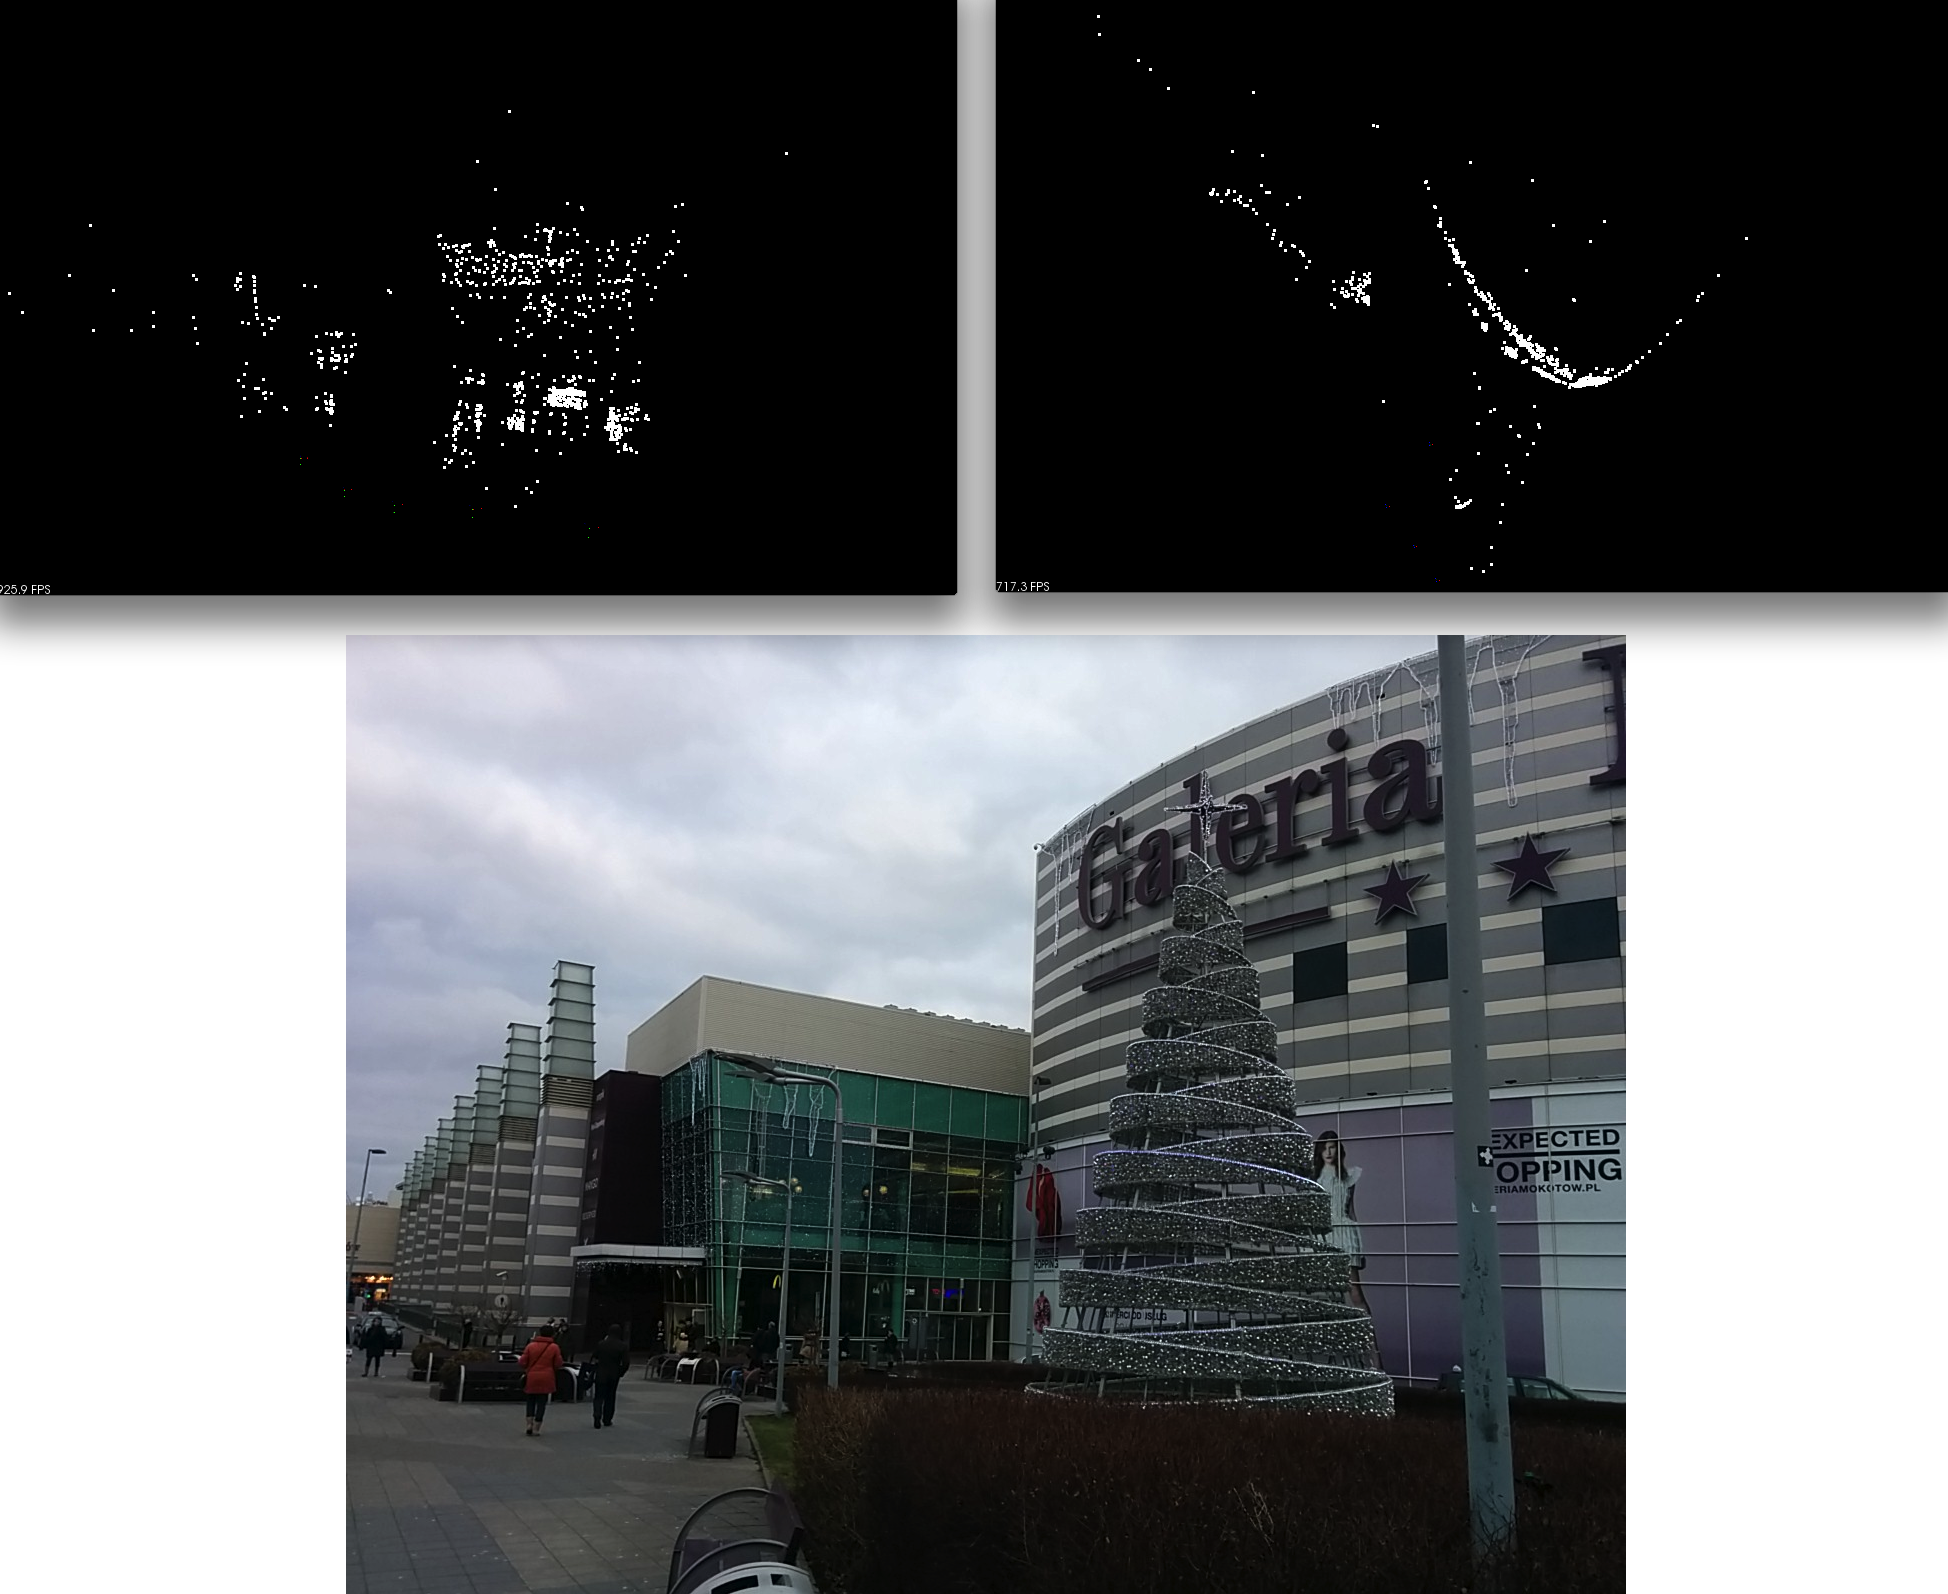
\includegraphics[width=\linewidth]{GallerFrontReconstruction}
    \caption[Reconstruction results of ''Gallery Front'' dataset]{Reconstruction results of ''Gallery Front'' dataset using rotation enhanced 8-point algorithm (left - front view, right - above view).}
\end{figure}


% ---------------------------------------------------------------------------
%: ----------------------- end of thesis sub-document ------------------------
% ---------------------------------------------------------------------------



 






